\section{Experiments}

\subsection{Phase 0~\textendash{}~Pipeline Setup}
\begin{frame}[fragile]{Phase 0~\textendash{}~Pipeline Setup}
    \begin{columns}[T]
        \begin{column}{0.56\textwidth}
            \begin{figure}
                \begin{minted}[style=friendly,fontsize=\scriptsize]{c}
imu_ids: [0, 1, 2, 3, 4, 5]
key_codes: [21, 22, 23, 34, ...]
sequence_length: 16

epochs: 0 //infinite
learning_rate: 0.002
batch_size: 100
sampling_rate: 25

network_type: cnn2d
cost_function: mse

convolution_n_filters: 50
convolution_filter_size: [3, 3]
convolution_n_pairs: 2
convolution_arr_dense: [10]
                \end{minted}
% training_ratio: 0.8
% output_threshold: 0.5
% n_hidden: 20
               \label{fig:config}
               \caption{Example of a configuration file (truncated)}
            \end{figure}
        \end{column}
        \begin{column}{0.38\textwidth}
            \begin{itemize}
                \item easily adjustable
                \item repeatable experiments
            \end{itemize}
        \end{column}
    \end{columns}
    \notes{
        \item Theano is a scientific mathematical library
        \begin{itemize}
            \item large scale calculations
            \item often numpy arrays
        \end{itemize}
        \item Lasagne is a ML-Framework based on Theano
        \begin{itemize}
            \item focused on Neural Networks
        \end{itemize}
    }
\end{frame}


\subsection{Phase 1~\textendash{}~Slow Single Finger}
\begin{frame}[fragile]{Phase 1~\textendash{}~Slow Single Finger}{Overview}
    \phasekeyboard{1}
    1 finger, 2 keys

    \pause
    \vspace{2em}
    Goals:
    \begin{itemize}
        \item detect keystrokes, ignore idle pose
        \item distinguish between close keys
        \item evaluate the configuration of the CNN
    \end{itemize}

    \notes{
        \item index finger moving between N, H
        \item pauses
        \item mostly detect pressed N
        \item always ignore H
    }
\end{frame}

\begin{frame}[fragile]{Phase 1~\textendash{}~Slow Single Finger}{Accuracy and Cost Function}
    \phasekeyboard{1}
        \begin{figure}
            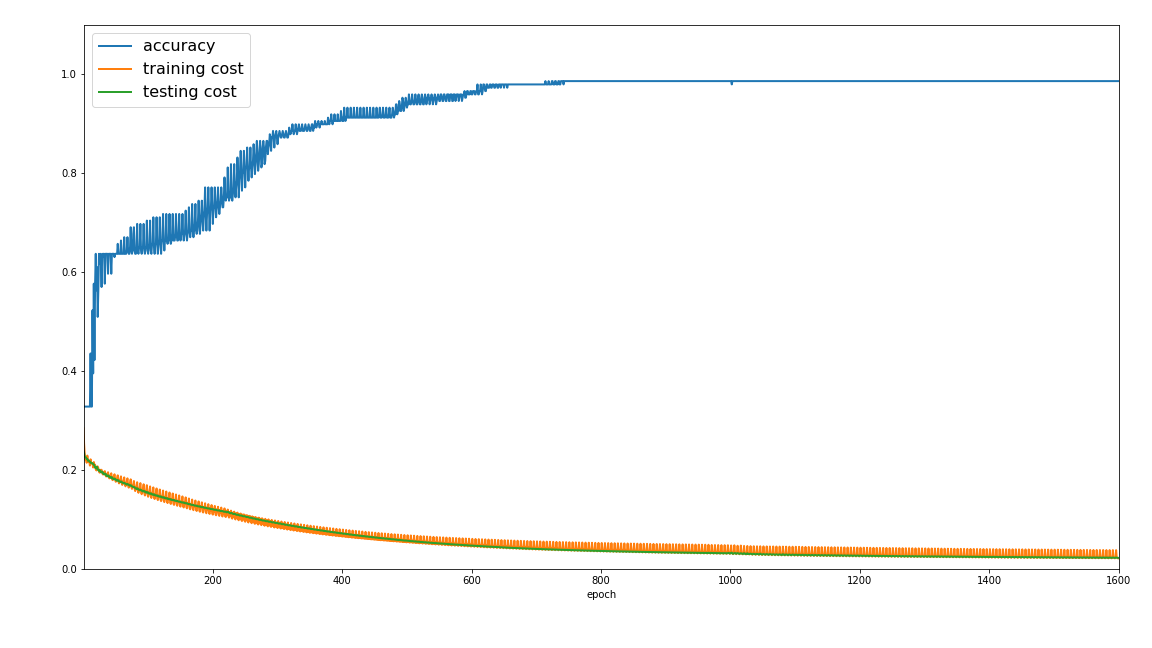
\includegraphics[width=0.85\textwidth]{../common/images/phase-1}
            \label{fig:phase11}
            \caption{Test results in the first $1 600$ epochs of learning phase 2}
        \end{figure}
    \notes{
        \item $1600$ epochs
        \item accuracy: amount of correctly classified samples
        \item 1 epoch: 1 batch
        \item 1 batch: 100 samples
        \item 1 sample: 1keystroke or nokey: 16 timesteps
    }
\end{frame}

\subsection{Phase 2~\textendash{}~Slow Multiple Fingers}
\begin{frame}[fragile]{Phase 2~\textendash{}~Slow Multiple Finger}{Overview}
    \phasekeyboard{2}
    3 fingers, 10 keys

    \pause
    \vspace{2em}
    Goals:
    \begin{itemize}
        \item distinguish between fingers
        \item handle hand movement
    \end{itemize}
\end{frame}

\begin{frame}[fragile]{Phase 2~\textendash{}~Slow Multiple Fingers}{Accuracy and Cost Function}
    \phasekeyboard{2}
    \begin{figure}
        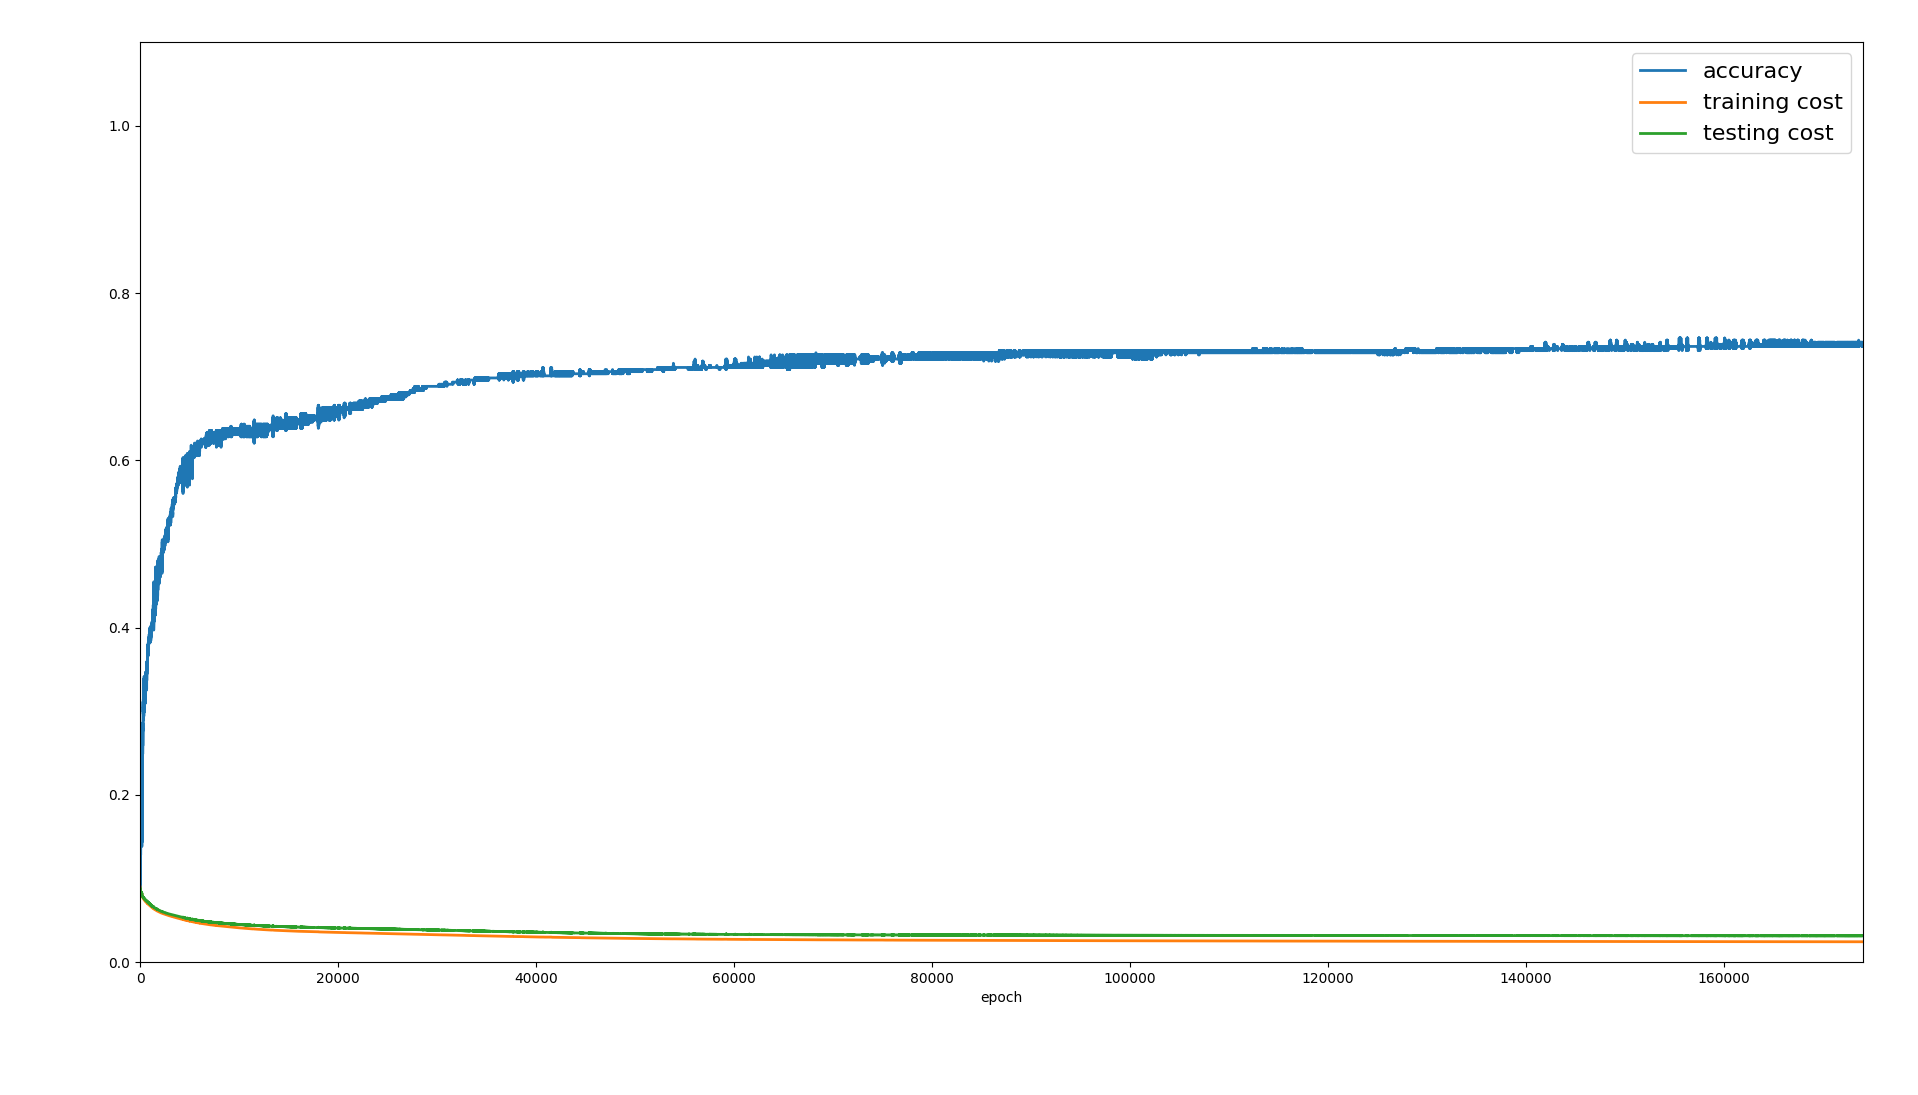
\includegraphics[width=0.85\textwidth]{../common/images/phase-2}
        \label{fig:phase21}
        \caption{Test results in the first $160 000$ epochs of learning phase 2}
    \end{figure}
    \notes{
        \item over $160000$ epochs $\rightarrow$ much more epochs necesarry
        \item accuracy only near 70\%
    }
\end{frame}

\subsubsection{Evaluation of Predictions}
\begin{frame}{Phase 2~\textendash{}~Slow Multiple Fingers}{Evaluation of Predictions}
    \phasekeyboard{2}
    \begin{figure}
        \scalebox{0.9}{
            \pgfkeys{/pgf/declare function={rescale(\x) = (\x*2-1)^3*0.5+0.5;}}

\begin{tikzpicture}[
    square/.style={
        inner sep=0pt,
        rectangle,
        minimum width=1cm,
        minimum height=0.5cm,
        anchor=north west,
    },
    every node/.style={
        font=\scriptsize,
    },
]
    % \node[inner sep=2pt,circle,fill=green] at (0, 0) {};
    \node[inner sep=0pt,rectangle,anchor=south east,rotate=90,minimum width=5cm,minimum height=0.5cm,draw,xshift=0.5\pgflinewidth,thick]
        at (0, -0.5) {\bfseries{}Actual};
    \node[inner sep=0pt,rectangle,anchor=south west,minimum width=10cm,minimum height=0.5cm,draw,xshift=-0.5\pgflinewidth,thick]
        at (1, 0) {\bfseries{}Predicted};

    \foreach \row [count=\y] in {{0,13,5,9,5,121,2,6,3,0},{0,175,0,0,0,0,0,0,0,0},{0,1,167,0,0,0,0,0,0,0},{0,0,0,181,0,0,0,0,0,0},{0,1,5,0,1,169,0,0,0,0},{0,0,1,0,1,215,0,3,0,0},{0,0,0,0,0,0,167,0,0,0},{0,0,0,0,0,0,0,180,0,0},{0,0,0,0,0,0,0,0,190,0},{0,0,0,0,4,178,1,0,0,0}} {
        \foreach \v [count=\x] in \row {
            \pgfmathsetmacro{\tmp}{\v/215.0}
            \pgfmathtruncatemacro{\back}{rescale(\tmp)*100}
            \pgfmathtruncatemacro{\fore}{(\tmp>0.5)*100}
            \node[square,fill=black!\back!white,text=white!\fore!black] at (\x,-\y*0.5) {$\v$};
        }
    }

    \foreach \key [count=\i] in {$\emptyset$,Y,U,G,H,J,B,N,M,\textvisiblespace} {
        \node[square] at (0, -(\i*0.5) {\bfseries\key};
        \node[square] at (\i, 0) {\bfseries\key};
    }

    \foreach \i in {2,...,10} {
        \draw[draw,dotted] (\i, 0) -- (\i, -5.5);
        \draw[draw,dotted] (0, -\i*0.5) -- (11, -\i*0.5);
    }

    \foreach \i in {1,11} {
        \draw[draw,thick] (\i, 0) -- (\i, -5.5);
        \draw[draw,thick] (0, -\i*0.5) -- (11, -\i*0.5);
    }
\end{tikzpicture}

        }
        \label{fig:confusion-matrix}
        \caption{Confusion matrix\citep{poole-artificial-intelligence}. From this we calculate the accuracy and per key recall \& precision \citep{davis2006}}
    \end{figure}

    \note{
        \begin{itemize}
            \item left : actual, right: predicted
            \item wrong classificated:
            \begin{itemize}
                \item no key as j
                \item h as j
                \item space as j
            \end{itemize}
            \item apple keyboard doesnt need much finger movement to press key
            \item $\rightarrow$ mechanical keyboard??!
            \item additional stuff:
            \begin{itemize}
                \item recall precision needs to be balenced (--> imbalanced data!!)
                \item recall: RECALL :D avoid FN!
                \item precision: avoid FP
                \item accuracy: TP / ALL
                \item recall:  TP/ TP +  FN how many relevant items (TP + FN) are selected
                \item precision: TP/ TP + FP how many selected items are relevant
            \end{itemize}
        \end{itemize}
    }
\end{frame}

\subsection{Phase 3~\textendash{}~Fast Typing}
\begin{frame}[fragile]{Phase 3~\textendash{}~Fast Typing}{Overview}
    \phasekeyboard{3}
    5 fingers, 27 keys

    \pause
    \vspace{2em}
    Goals:
    \begin{itemize}
        \item recognizing every righthand key stroke
        \item achieve high accuracy
        \item learn a robust model
        \item fluent typing
    \end{itemize}

    \notes{
        \item future (we did not do this yet)
        \item next step: online learning
        \item modification of movements
    }
\end{frame}
